\section{The Direct and Indirect Effects of Health Insurance}
\label{sec:healthinsurance}


\begin{figure}[h!]
    \caption{Effects of Health Insurance in the Oregon Health Insurance Experiment.}
    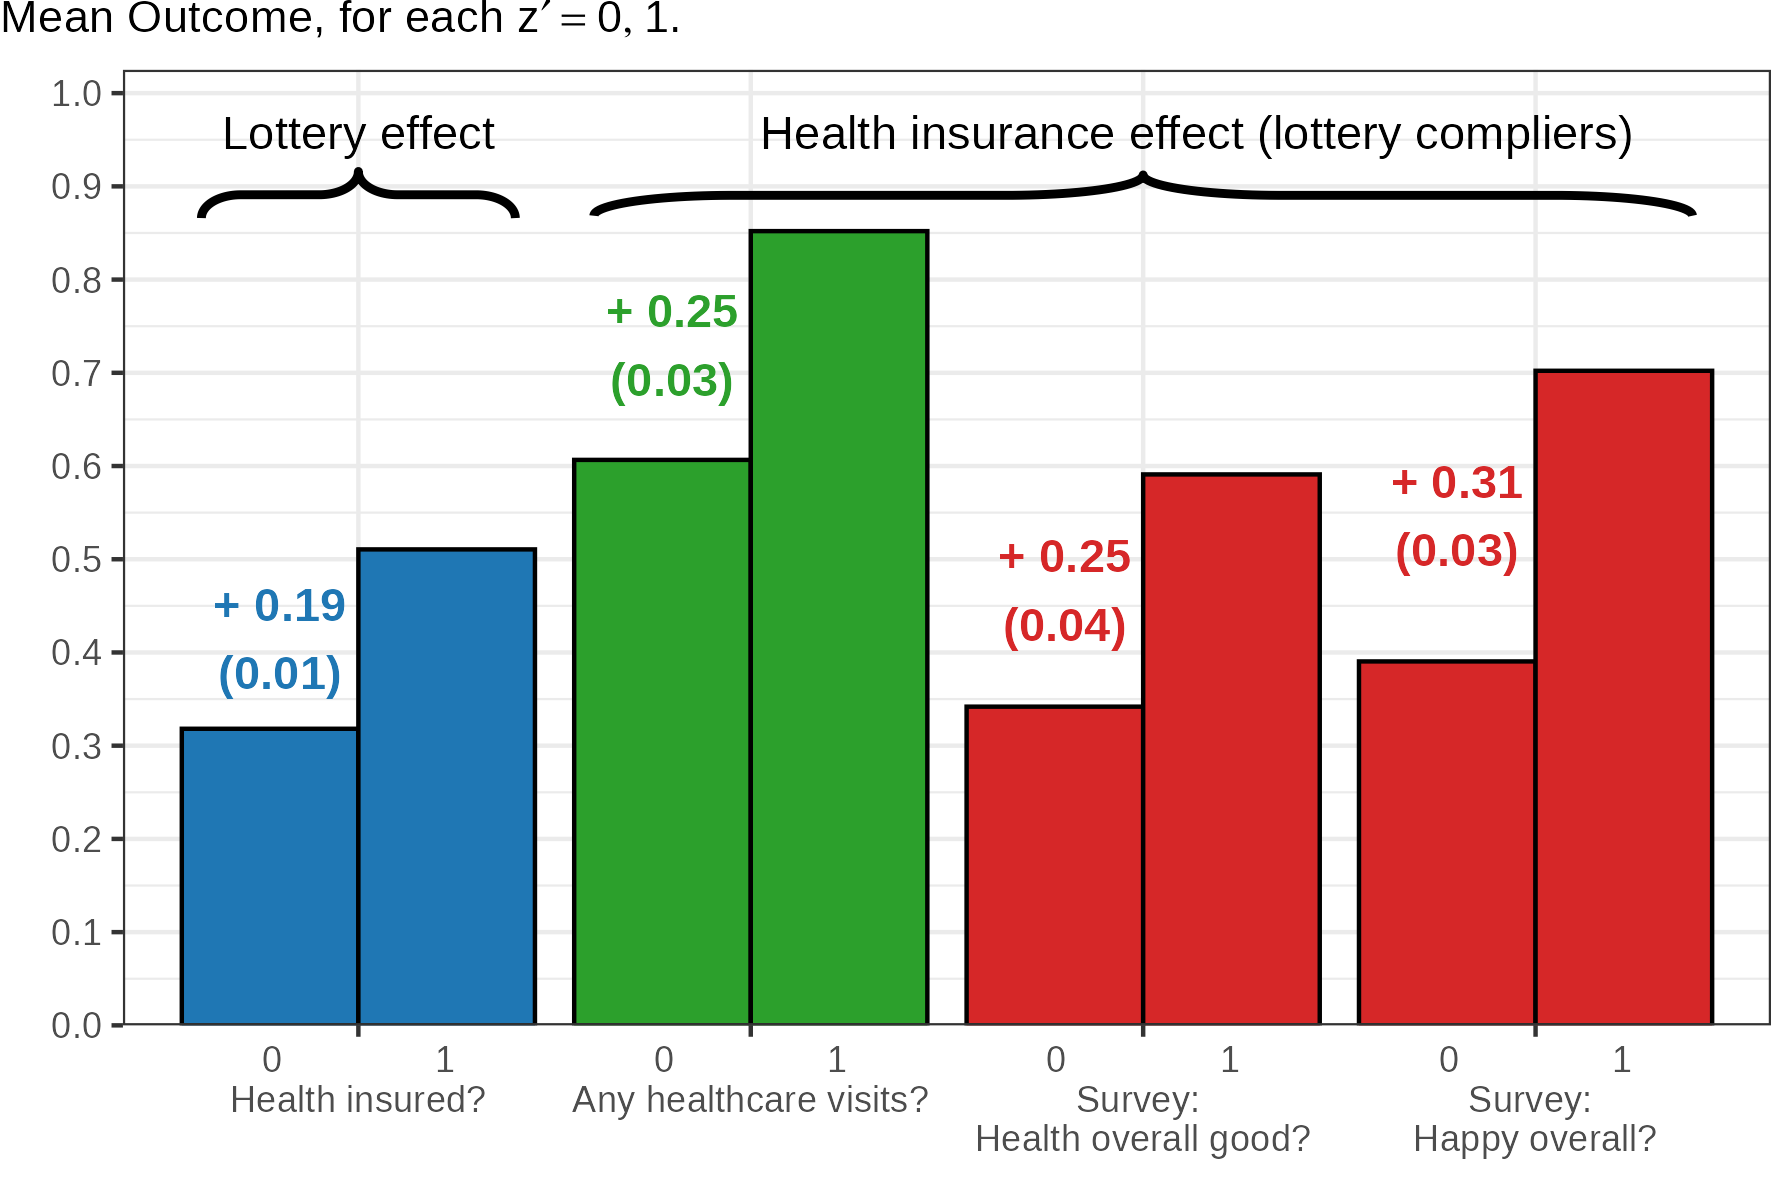
\includegraphics[width=\textwidth]{figures/insurance-effects.png}
    \label{fig:healthinsurance-effects}
    \justify
    \footnotesize    
    \textbf{Note:}
    This figure summarises the pertinent results of the Oregon Health Insurance Experiment \citep{finkelstein2008oregon}.
    The lottery results show that being randomly selected off the Medicaid wait-list increased health insurance rate by 19\%.
    The effect of health insurance shows estimates of the avaerage complier effect, using the lottery as an instrument for having health insurance and the \cite{abadie2003semiparametric} weighting scheme to estimate the average complier levels $\E{Y_i(., d')}{\text{lottery complier}}$ for $d'=0,1$.
\end{figure}
